\begin{frame}
  \frametitle{Diversion Detection with Cyclus}
  	\textbf{Motivation}
        \begin{itemize}
                \item Safeguard by design
                \item Model diversion inside facilities
                \item transition from LWR to SFR
        \end{itemize}
    \textbf{Goals}
    	\begin{itemize}
    		\item Detect diversion using signatures and observables.
    		\item Optimum detector and inspection locations in pyroprocessing
    		\item Characterize detection sensitivities and false positive rates
    	\end{itemize}
  \begin{figure}
    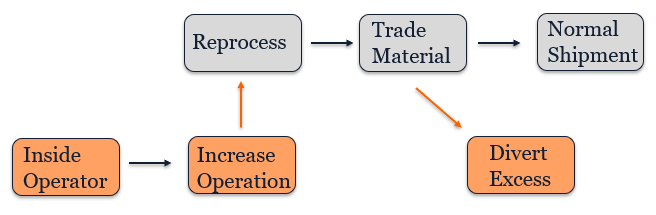
\includegraphics[width=0.7\linewidth]{./images/westphal-diversion}
    \caption{Operator vs nefarious diversion.}
    \label{fig:diversion}
  \end{figure}
\end{frame}

\begin{frame}
	\frametitle{PyRe Archetype}
	\begin{columns}
		\column[t]{6cm}
		\begin{itemize}
			\item Facility containing multiple sub-processes:
			\begin{itemize}
				\item Separately handled.
				\item Independent transactions, possibility of diversion.
			\end{itemize}
			\item Operation setting impact efficiency.
			\item Generic facility:
			\begin{itemize}
				\item Multiple types of pyro plants.
				\item LWR vs SFR.
			\end{itemize}
		\end{itemize}
		\begin{block}{Diversion Detection}
			Material transactions are no longer a reliable method. Instead we use
			signatures and observables:
			\begin{itemize}
				\item Temperature, power draw, etc.
			\end{itemize}
			A Cumulative Sum change algorithm is used to detect any significant changes.
		\end{block}
		\column[t]{5cm}
		\begin{figure}
			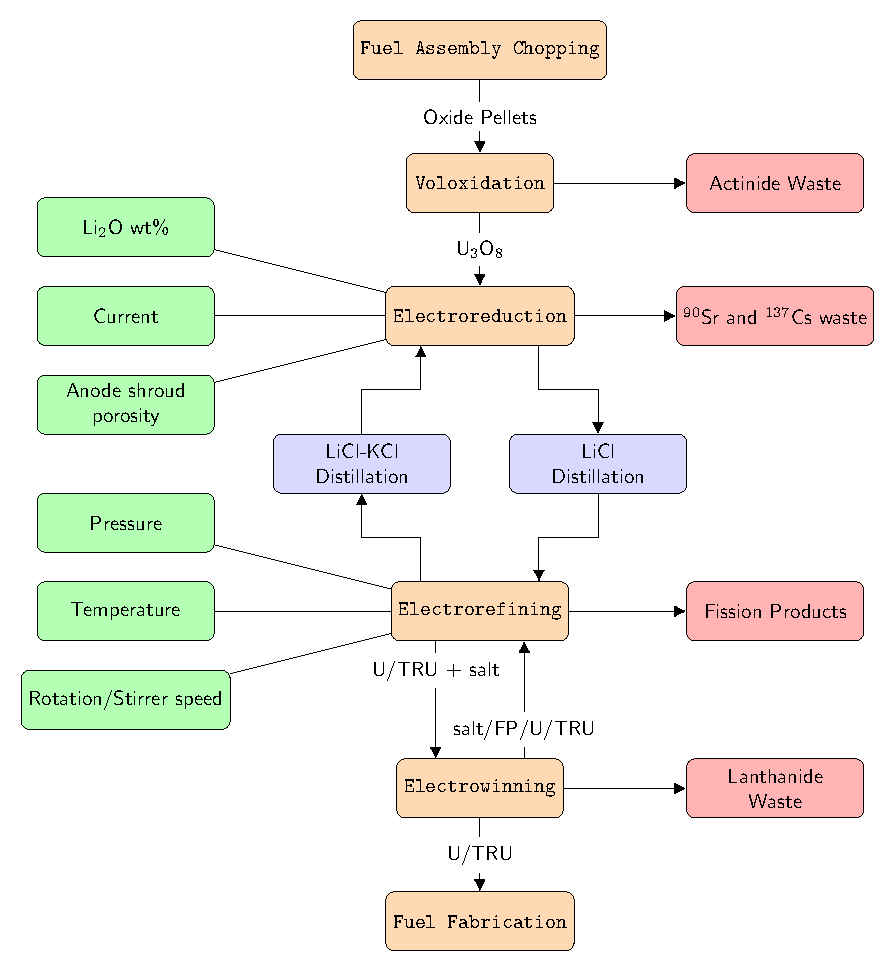
\includegraphics[width=\linewidth]{./images/westphal-pyre.pdf}
			\caption{PyRe flow diagram for LWR waste configuration.}
			\label{fig:pyre}
		\end{figure}
	\end{columns}
\end{frame}